\documentclass[conference,11pt]{IEEEtran}
\usepackage[utf8]{inputenc}
\usepackage[english]{babel}
\usepackage[left=1in,right=1in,top=1in,bottom=1in,footskip=.25in]{geometry}
\usepackage{cite}
\usepackage{hyperref}
\usepackage{fancyhdr}
\usepackage{datetime}
\usepackage{amsmath}
\usepackage{url}
\usepackage{subfig}
\usepackage{float}
\usepackage{graphicx}
\graphicspath{ {images/} }
\usepackage{setspace}
%\setlength{\parskip}{1em}
\pagenumbering{arabic}
\pagestyle{fancy}
\usepackage{pbox}
% excel2latex
\usepackage{multirow}
\usepackage{xcolor}
\usepackage{colortbl}
\usepackage{rotating}
\usepackage{booktabs,arydshln}

\makeatletter
\def\adl@drawiv#1#2#3{%
        \hskip.5\tabcolsep
        \xleaders#3{#2.5\@tempdimb #1{1}#2.5\@tempdimb}%
                #2\z@ plus1fil minus1fil\relax
        \hskip.5\tabcolsep}
\newcommand{\cdashlinelr}[1]{%
  \noalign{\vskip\aboverulesep
           \global\let\@dashdrawstore\adl@draw
           \global\let\adl@draw\adl@drawiv}
  \cdashline{#1}
  \noalign{\global\let\adl@draw\@dashdrawstore
           \vskip\belowrulesep}}
\makeatother

\usepackage[numbered,framed]{matlab-prettifier}
\usepackage[T1]{fontenc}
\usepackage[scaled]{beramono}
\lstset{
  style              = Matlab-editor,
  basicstyle         = \mlttfamily,
  escapechar         = ",
  mlshowsectionrules = true,
}

\title{Accurate, scalable microbiome quantification with shallow shotgun sequencing}
\author{
    \IEEEauthorblockN{Benjamin Hillmann}
    \IEEEauthorblockA{
        \today
    }
}

\begin{document}
\onecolumn
\maketitle

\begin{abstract}

Despite the association of microbial communities with many aspects of human, environmental, plant, and animal health, there exists no cost-efficient method for precisely characterizing the species and genes present in a microbial community. Current methods that use affordable amplicon sequencing techniques cannot resolve taxonomy past the genus level and only can classify clades whose genome has the marker gene. While deep whole-genome shotgun (WGS) is able to solve these problems, the technique is prohibitively expensive for large-scale studies. To address these issues, we propose a novel computational pipeline SHOGUN using shallow whole-genome shotgun (shallow shotgun) sequencing that recovers accurate taxonomic profiles of human microbiomes. We show that by sequencing at fraction of the cost and depth of WGS surveys, we can provide nearly the same measured species-level taxonomic profile. We demonstrate the shallow shotgun results on multiple real biological datasets and simulated communities. The pipeline SHOGUN relies on whole-genome reference databases, and is therefore most useful for well-characterized environments such as the human microbiomes in the gut, skin or oral cavity. Thus, SHOGUN allows researchers to obtain near-WGS data quality at only slightly higher cost than amplicon sequencing, enabling a fundamental shift toward higher precision in human microbiome research.

\end{abstract}

\section{Introduction}

Microbial community structure is associated with many aspects of human, plant, animal, and environmental health; despite this, there are currently no affordable methods to characterize what species and genes are present in a given community \cite{prifti_new_2013}. Unfortunately, most of the microbes in these communities cannot be cultured, so to observe the biological contents of these communities we must quantify their taxonomic profiles through sequencing the microbes DNA. This has led to a dramatic influx of large metagenomic datasets and a surge in the demand for scientists to precisely describe the species within these communities to determine which organisms are beneficial and which are detrimental for different environments and applications.

Microbiome DNA analysis is typically performed in one of two ways: using amplicon-based (16S) or whole-genome shotgun-based (WGS) sequencing methods. Amplicon based techniques typically amplify a highly variable region of the 16S ribosomal RNA gene, although other genes may be targeted in particular cases, such as for fungal microbiome sequencing. Amplicon sequencing is affordable, but often cannot distinguish between species due to sequence similarities, and does not allow high-accuracy prediction of the functional repertoire. Because amplicon methods rely on DNA primers to amplify the region of interest, they are also subject to high levels of bias and can fail to capture organisms whose DNA sequence does not match the primers. As an alternative, WGS sequencing sequences randomly selected fragments of all DNA present in a microbiome. WGS directly measures the functional repertoire of the microbiome by capturing a snapshot of the total metagenomic content and allows strain-level characterization of microbiomes by mapping reads to the unique markers of strain reference genomes. WGS, however, is typically ten times more expensive than amplicon sequencing due to its use of costly library preparation protocols and and the additional costs of very deep sequencing. This forces researchers to choose between affordability with amplicon methods, and accuracy with WGS.

A major concern for the use of any taxonomic quantification profile is having the ability to identify and quantify distinct taxonomic clades from within a complex community. If a strain is able to be grown in a monoculture or isolated, deep coverage of its genome allows precise assembly and annotation of its strain-specific polymorphisms (SNP), functional genes and other higher level functional modules. The assembled genomes and annotations are then placed in a database \cite{tatusova_refseq_2014}, and can be utilized as a reference genome for taxonomic profiling. In mixed microbial communities, such as the human gut microbiome, a WGS survey has been shown to be effective at recovering the species-to-strain specific taxonomic profile of the community. However, as previously mentioned, WGS are prohibitively expensive due to the high sequencing depth required for coverage of genome assembly, traditional low multiplexing of samples submitted to be sequenced, and SNP detection in individual strains. The goal of microbiome surveys is not always for the assembly of individual strains, but often is looking for differential microbial communities between disease states. Due to this goal, the exploration of accurate species level taxonomic profiles at varying shotgun sequencing depths should be explored to reduce costs of research with different objectives.

Development of robust yet affordable methods for accurate microbial profiling is a major priority for the microbiome research field. The critical barriers to quantifying microbiomes at the species level that are affordable, accurate and reproducible. Overcoming the shortcomings of amplicon and shotgun techniques presents major challenges in the field of metagenomics, and prevents scientists from performing highly precise, large-scale studies. After microbial communities have been sequenced, it is the objective of the researcher to utilize informatics methods to correlate the taxonomic and functional profiles of a sample to a trait of interest. However, these methods operate under the assumption that the underlying taxonomic and functional profiling are accurate. If methods are developed to more accurately identify the profiles of a community, the increased precision will cascade down every step along the metagenomics pipeline. With more precise profiles, the informatics methods will have more power to test hypotheses and better ability detect the causal role these communities play. Accurate cost- and time-effective taxonomic quantification of environmental samples is essential. Given the weaknesses of the aforementioned techniques, we propose novel highly data-efficient methods for species- and strain-level resolution taxonomic and functional profiles in low-depth shotgun metagenomic datasets (shallow shotgun).

Here we describe a novel approach using shallow shotgun sequencing, combined with our proposed shallow shotgun (SHOGUN) analysis pipeline \cite{benjamin_hillmann_knights-lab/shogun:_2017}, as an alternative to WGS sequencing. We show through analysis of several biological data sets and through simulated data that SHOGUN provides nearly the same accuracy at the species and functional level as deep WGS sequencing, but at a small fraction of the cost, with materials and DNA sequencing with comparable cost to amplicon sequencing. Thus, we expect that SHOGUN will allow researchers to switch immediately from marker gene sequencing to shallow shotgun sequencing for little additional cost and large accuracy payoff.

\section{Materials and Methods}


\subsection{Database}

%%% table:database_stats
\begin{table}[hbt]
  \centering
  \begin{tabular}{l|r|r}
      \textit{Kingdom} & \textit{Number of Genomes} & \textit{Megabases (Mbp)} \\ \hline
      Archaea & 238 & 627,101.26\\ \hline
      Bacteria & 4,884 & 19,308,087.26\\ \hline
      Plasmid & 614 & 198,476.94\\ \hline
      Viroids & 46 & 15.50\\ \hline
      Viruses & 7,194 & 253,668.36\\ \hline \hline
      \textbf{Total} & \textbf{12,976} & \textbf{20,387,349.32}\\ 
  \end{tabular}
  \label{table:database_stats}
\end{table}

The database of genomes for all analysis in this paper was all complete, representative Archaea, Bacteria, Plasmid, Viroids and Virus genomes from the reference database RefSeq version number 82 as of May 8, 2017 \cite{tatusova_refseq_2014}. The catalog for the genomes is available at \url{ftp://ftp.ncbi.nlm.nih.gov/refseq/release/release-catalog/archive/}, and the release statistics notes are available at \url{ftp://ftp.ncbi.nlm.nih.gov/refseq/release/release-notes/archive/RefSeq-release82.txt}. The statistics for our database

\subsection{Taxonomic Profilers}

A typical protocol for going from next-generation sequencing (NGS) reads of a mixed community to a taxonomic profile counts per clade is described in \textit{Figure~\ref{fig:shogun_pipeline}}. Depending on the taxonomic profile tool used, the steps in the protocol can vary widely. We chose to evaluate tools against our taxonomic profiler SHOGUN \cite{benjamin_hillmann_knights-lab/shogun:_2017} pipeline based on their ease of use and documentation, availability as an open-source tool, the ability to create a user defined database, summarize a taxonomy profile at the species level, and the ability to scale to large datasets with multiple threads per process. A summary of the taxonomic profilers selected and some pros and cons of each is described in \textit{Figure~\ref{fig:shogun_pipeline}}.

%%% fig:taxonomic_profiler
\begin{figure}[hbt]
    \centering
    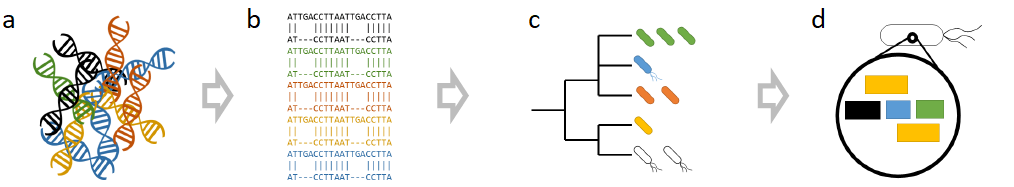
\includegraphics[width=0.8\linewidth]{fig/taxonomic_profiler.png}
    \caption{(a) Raw reads from the sequencing machine are demultiplexed into individual samples. Then, each read is quality controlled with by removing adapters, low quality bases and contaminates such as host reads \cite{consortium_structure_2012}. Optionally, the read pairs can be stitched \cite{magoc_flash:_2011}. (b) The quality-controlled reads are aligned against a database of known genomes to identify each read's most likely source taxon \cite{langmead_fast_2012}. (c) The taxa that are hit are filtered out and summarized at a specific level. These processing steps include last common ancestor assignment \cite{hong_pathoscope_2014}, genome coverage analysis \cite{wood_kraken:_2014}, and redistribution of reads to a specific taxonomic level \cite{lu_bracken:_2017}. (d) After the taxonomic prediction is set, the full functional repertoire of genes is directly observed through a bag-of-genes approach or predicted through a per microbe approach \cite{langille_predictive_2013}.}
      \label{fig:taxonomic_profiler}
\end{figure}

%%% fig:shogun_schematic
\begin{figure}[hbt]
    \centering
    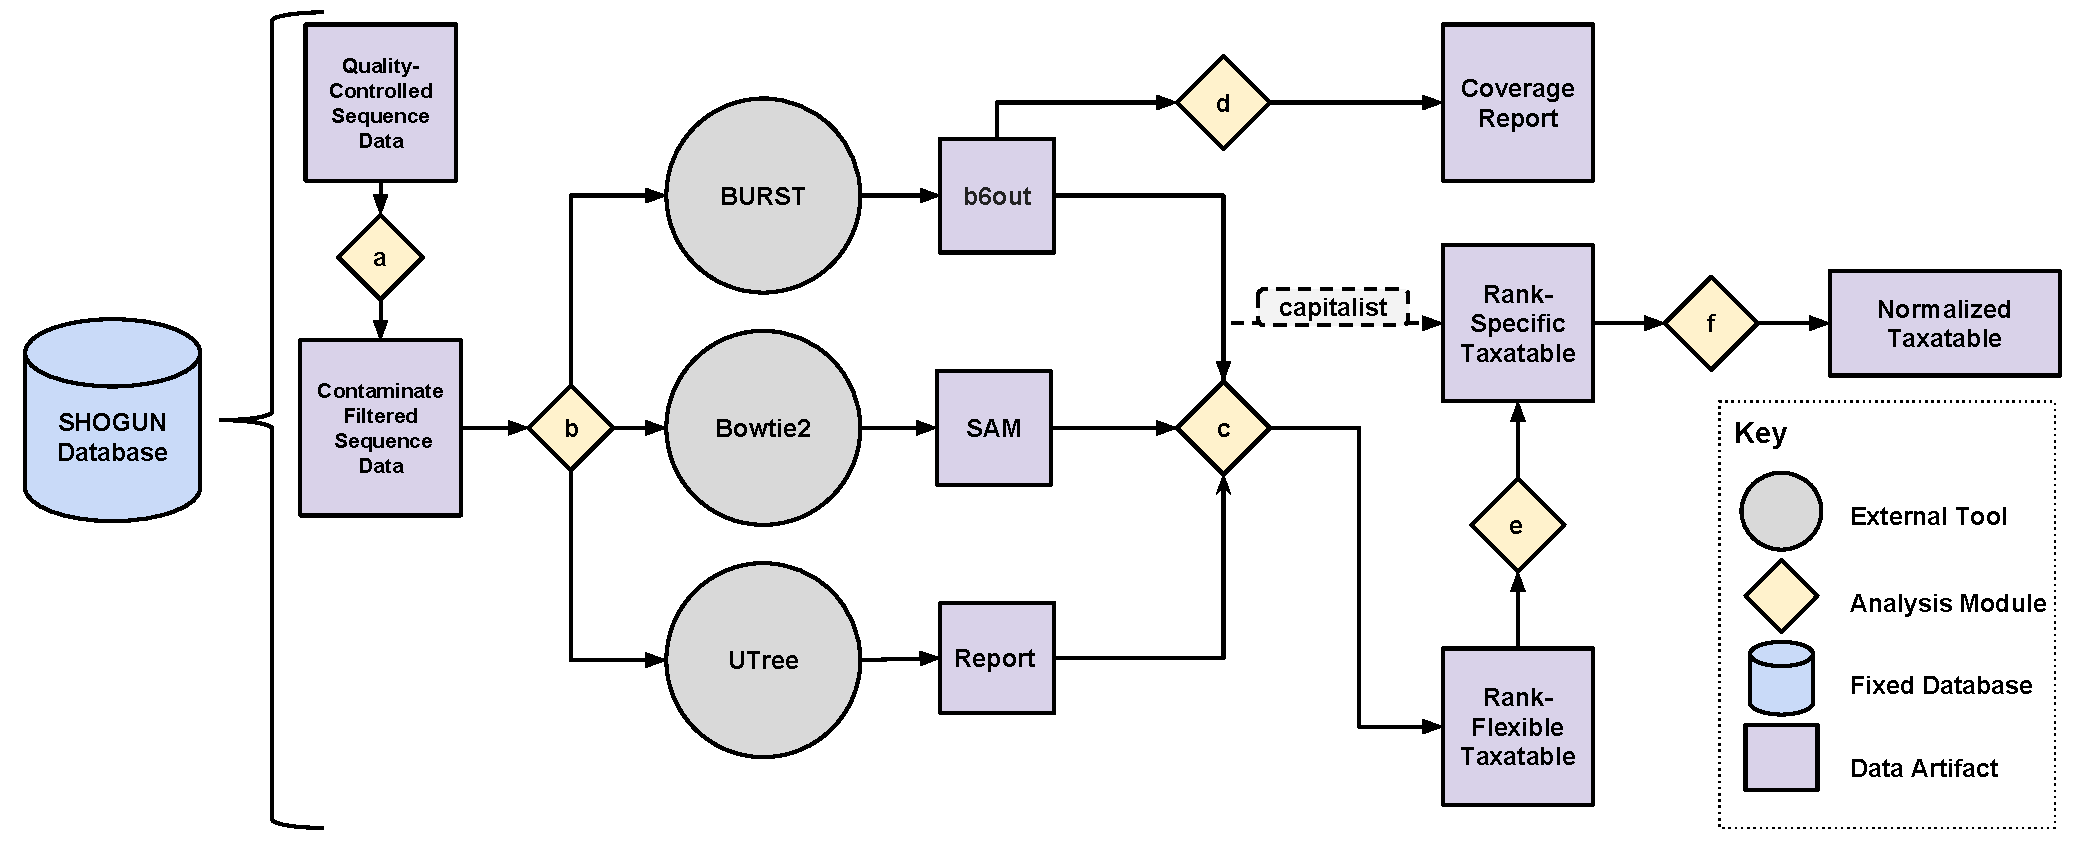
\includegraphics[width=0.8\linewidth]{fig/shogun_schematic.png}
    \caption{(a) Raw reads from the sequencing machine are demultiplexed into individual samples. Then, each read is quality controlled with by removing adapters, low quality bases and contaminates such as host reads \cite{consortium_structure_2012}. Optionally, the read pairs can be stitched \cite{magoc_flash:_2011}. (b) The quality-controlled reads are aligned against a database of known genomes to identify each read's most likely source taxon \cite{langmead_fast_2012}. (c) The taxa that are hit are filtered out and summarized at a specific level. These processing steps include last common ancestor assignment \cite{hong_pathoscope_2014}, genome coverage analysis \cite{wood_kraken:_2014}, and redistribution of reads to a specific taxonomic level \cite{lu_bracken:_2017}. (d) After the taxonomic prediction is set, the full functional repertoire of genes is directly observed through a bag-of-genes approach or predicted through a per microbe approach \cite{langille_predictive_2013}.}
      \label{fig:shogun_schematic}
\end{figure}

%%% fig:hmp_beta
\begin{figure}[hbt]
    \centering
    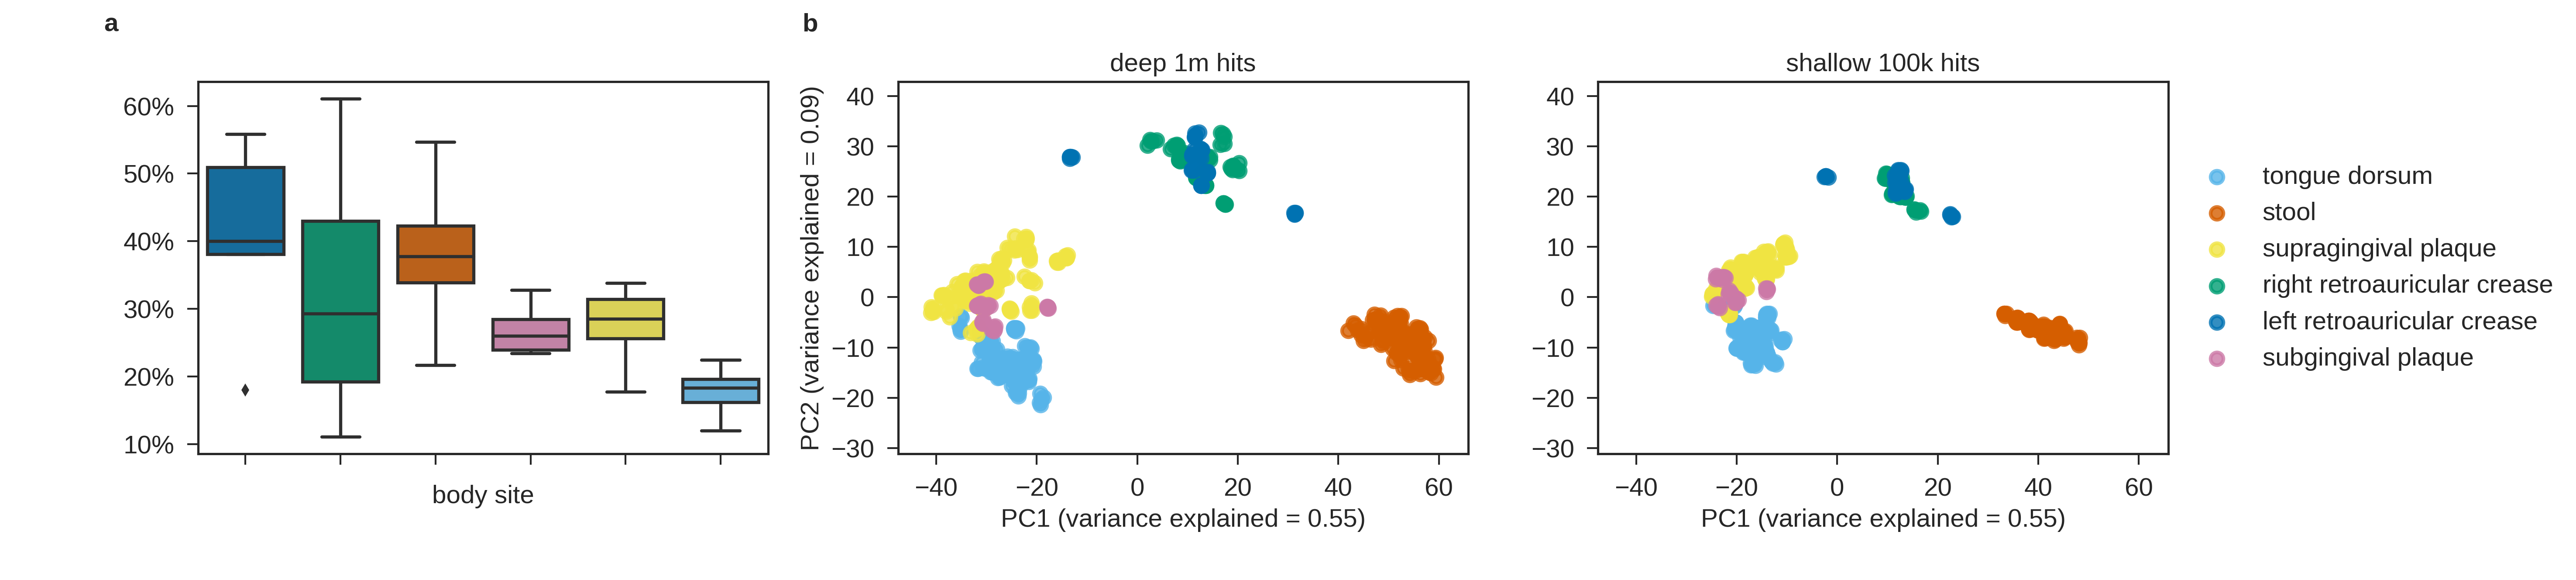
\includegraphics[width=0.8\linewidth]{fig/hmp_beta.png}
    \caption{(a) Raw reads from the sequencing machine are demultiplexed into individual samples. Then, each read is quality controlled with by removing adapters, low quality bases and contaminates such as host reads \cite{consortium_structure_2012}. Optionally, the read pairs can be stitched \cite{magoc_flash:_2011}. (b) The quality-controlled reads are aligned against a database of known genomes to identify each read's most likely source taxon \cite{langmead_fast_2012}. (c) The taxa that are hit are filtered out and summarized at a specific level. These processing steps include last common ancestor assignment \cite{hong_pathoscope_2014}, genome coverage analysis \cite{wood_kraken:_2014}, and redistribution of reads to a specific taxonomic level \cite{lu_bracken:_2017}. (d) After the taxonomic prediction is set, the full functional repertoire of genes is directly observed through a bag-of-genes approach or predicted through a per microbe approach \cite{langille_predictive_2013}.}
      \label{fig:hmp_beta}
\end{figure}

%%% fig:hmp_alpha
\begin{figure}[hbt]
    \centering
    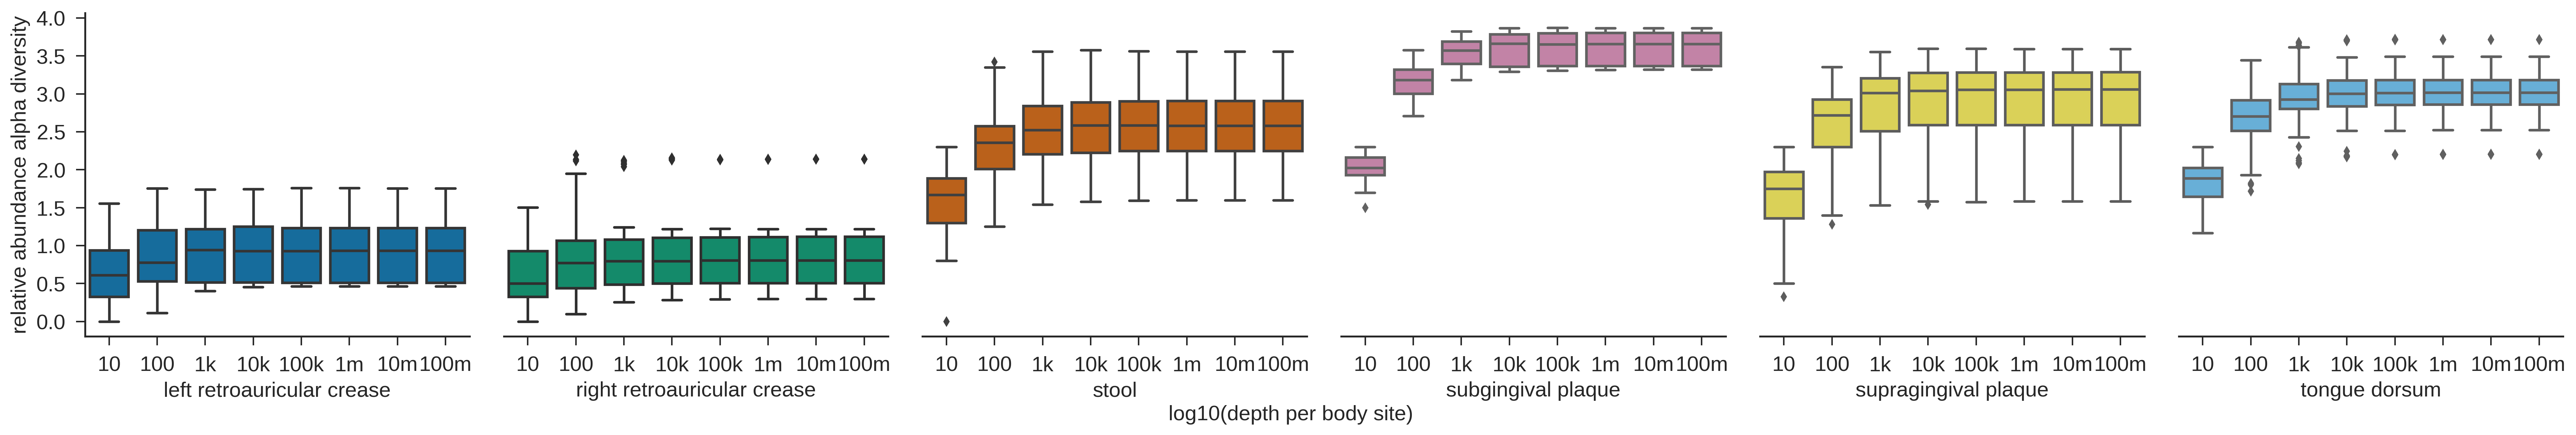
\includegraphics[width=0.8\linewidth]{fig/hmp_alpha.png}
    \caption{(a) Raw reads from the sequencing machine are demultiplexed into individual samples. Then, each read is quality controlled with by removing adapters, low quality bases and contaminates such as host reads \cite{consortium_structure_2012}. Optionally, the read pairs can be stitched \cite{magoc_flash:_2011}. (b) The quality-controlled reads are aligned against a database of known genomes to identify each read's most likely source taxon \cite{langmead_fast_2012}. (c) The taxa that are hit are filtered out and summarized at a specific level. These processing steps include last common ancestor assignment \cite{hong_pathoscope_2014}, genome coverage analysis \cite{wood_kraken:_2014}, and redistribution of reads to a specific taxonomic level \cite{lu_bracken:_2017}. (d) After the taxonomic prediction is set, the full functional repertoire of genes is directly observed through a bag-of-genes approach or predicted through a per microbe approach \cite{langille_predictive_2013}.}
      \label{fig:hmp_alpha}
\end{figure}

%%% fig:hmp_taxa
\begin{figure}[hbt]
    \centering
    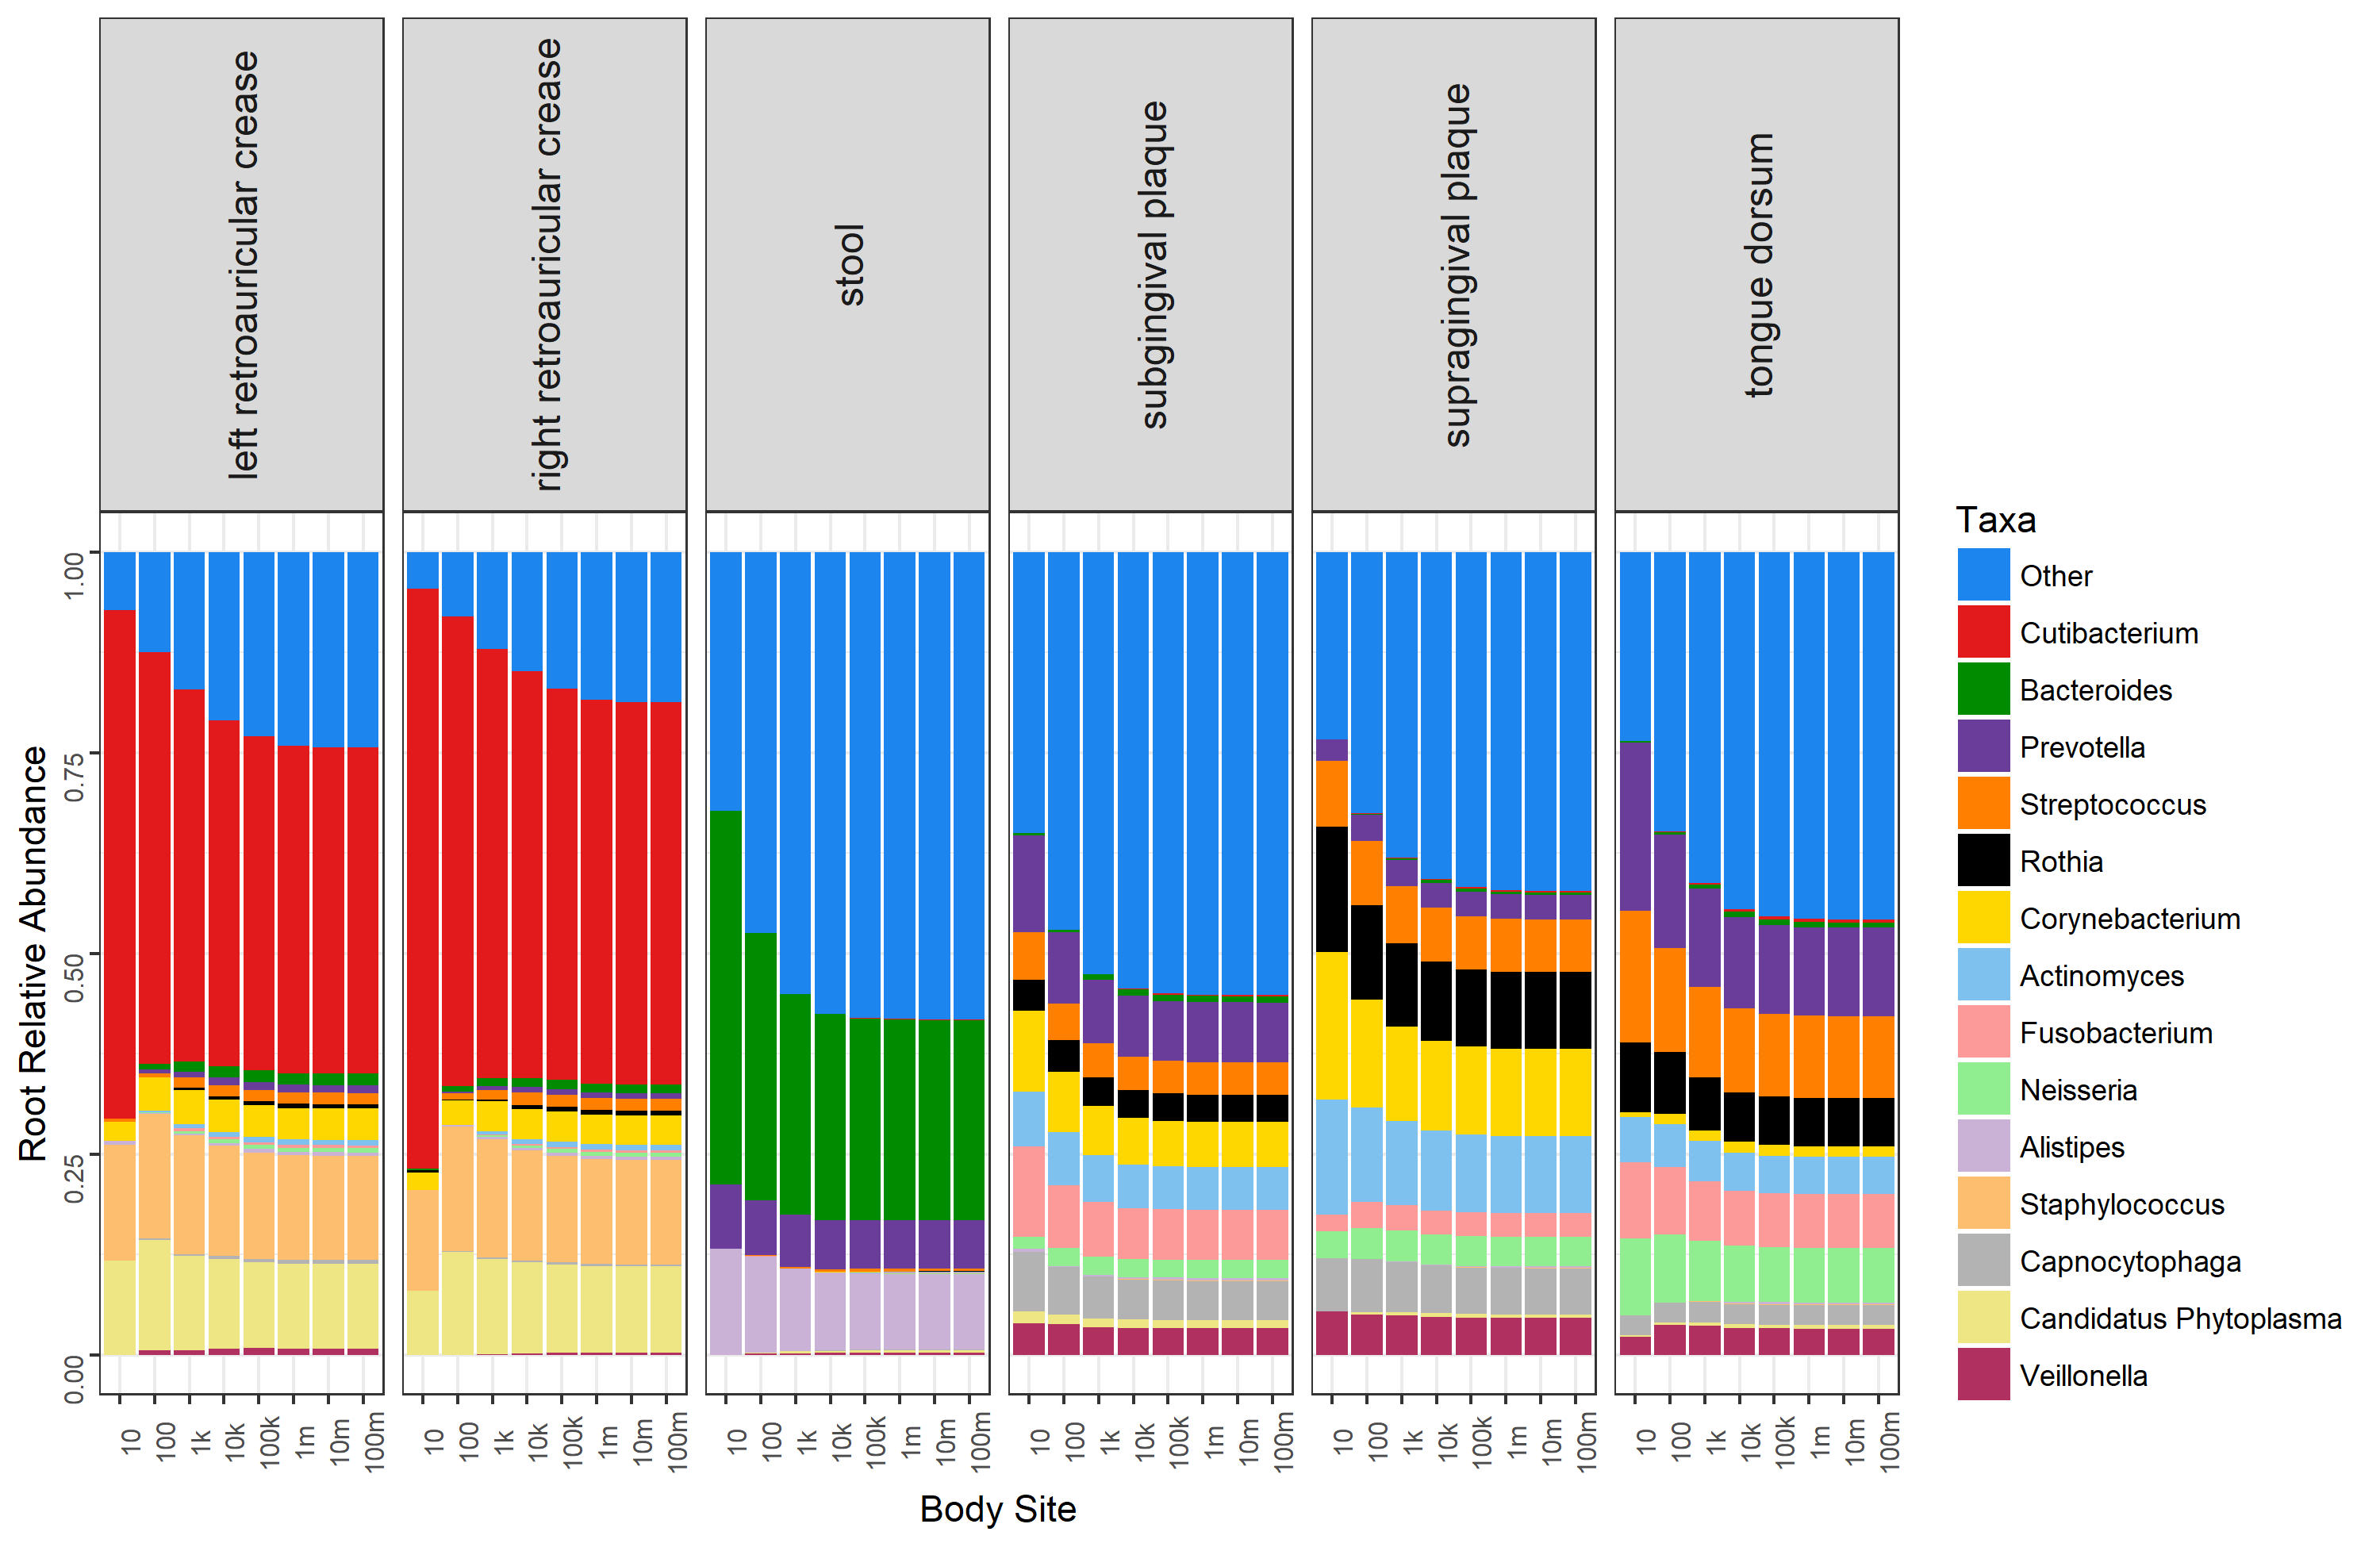
\includegraphics[width=0.8\linewidth]{fig/hmp_taxa.png}
    \caption{(a) Raw reads from the sequencing machine are demultiplexed into individual samples. Then, each read is quality controlled with by removing adapters, low quality bases and contaminates such as host reads \cite{consortium_structure_2012}. Optionally, the read pairs can be stitched \cite{magoc_flash:_2011}. (b) The quality-controlled reads are aligned against a database of known genomes to identify each read's most likely source taxon \cite{langmead_fast_2012}. (c) The taxa that are hit are filtered out and summarized at a specific level. These processing steps include last common ancestor assignment \cite{hong_pathoscope_2014}, genome coverage analysis \cite{wood_kraken:_2014}, and redistribution of reads to a specific taxonomic level \cite{lu_bracken:_2017}. (d) After the taxonomic prediction is set, the full functional repertoire of genes is directly observed through a bag-of-genes approach or predicted through a per microbe approach \cite{langille_predictive_2013}.}
      \label{fig:hmp_taxa}
\end{figure}

%%% fig:karlsson2013_f1_combined
\begin{figure}[hbt]
    \centering
    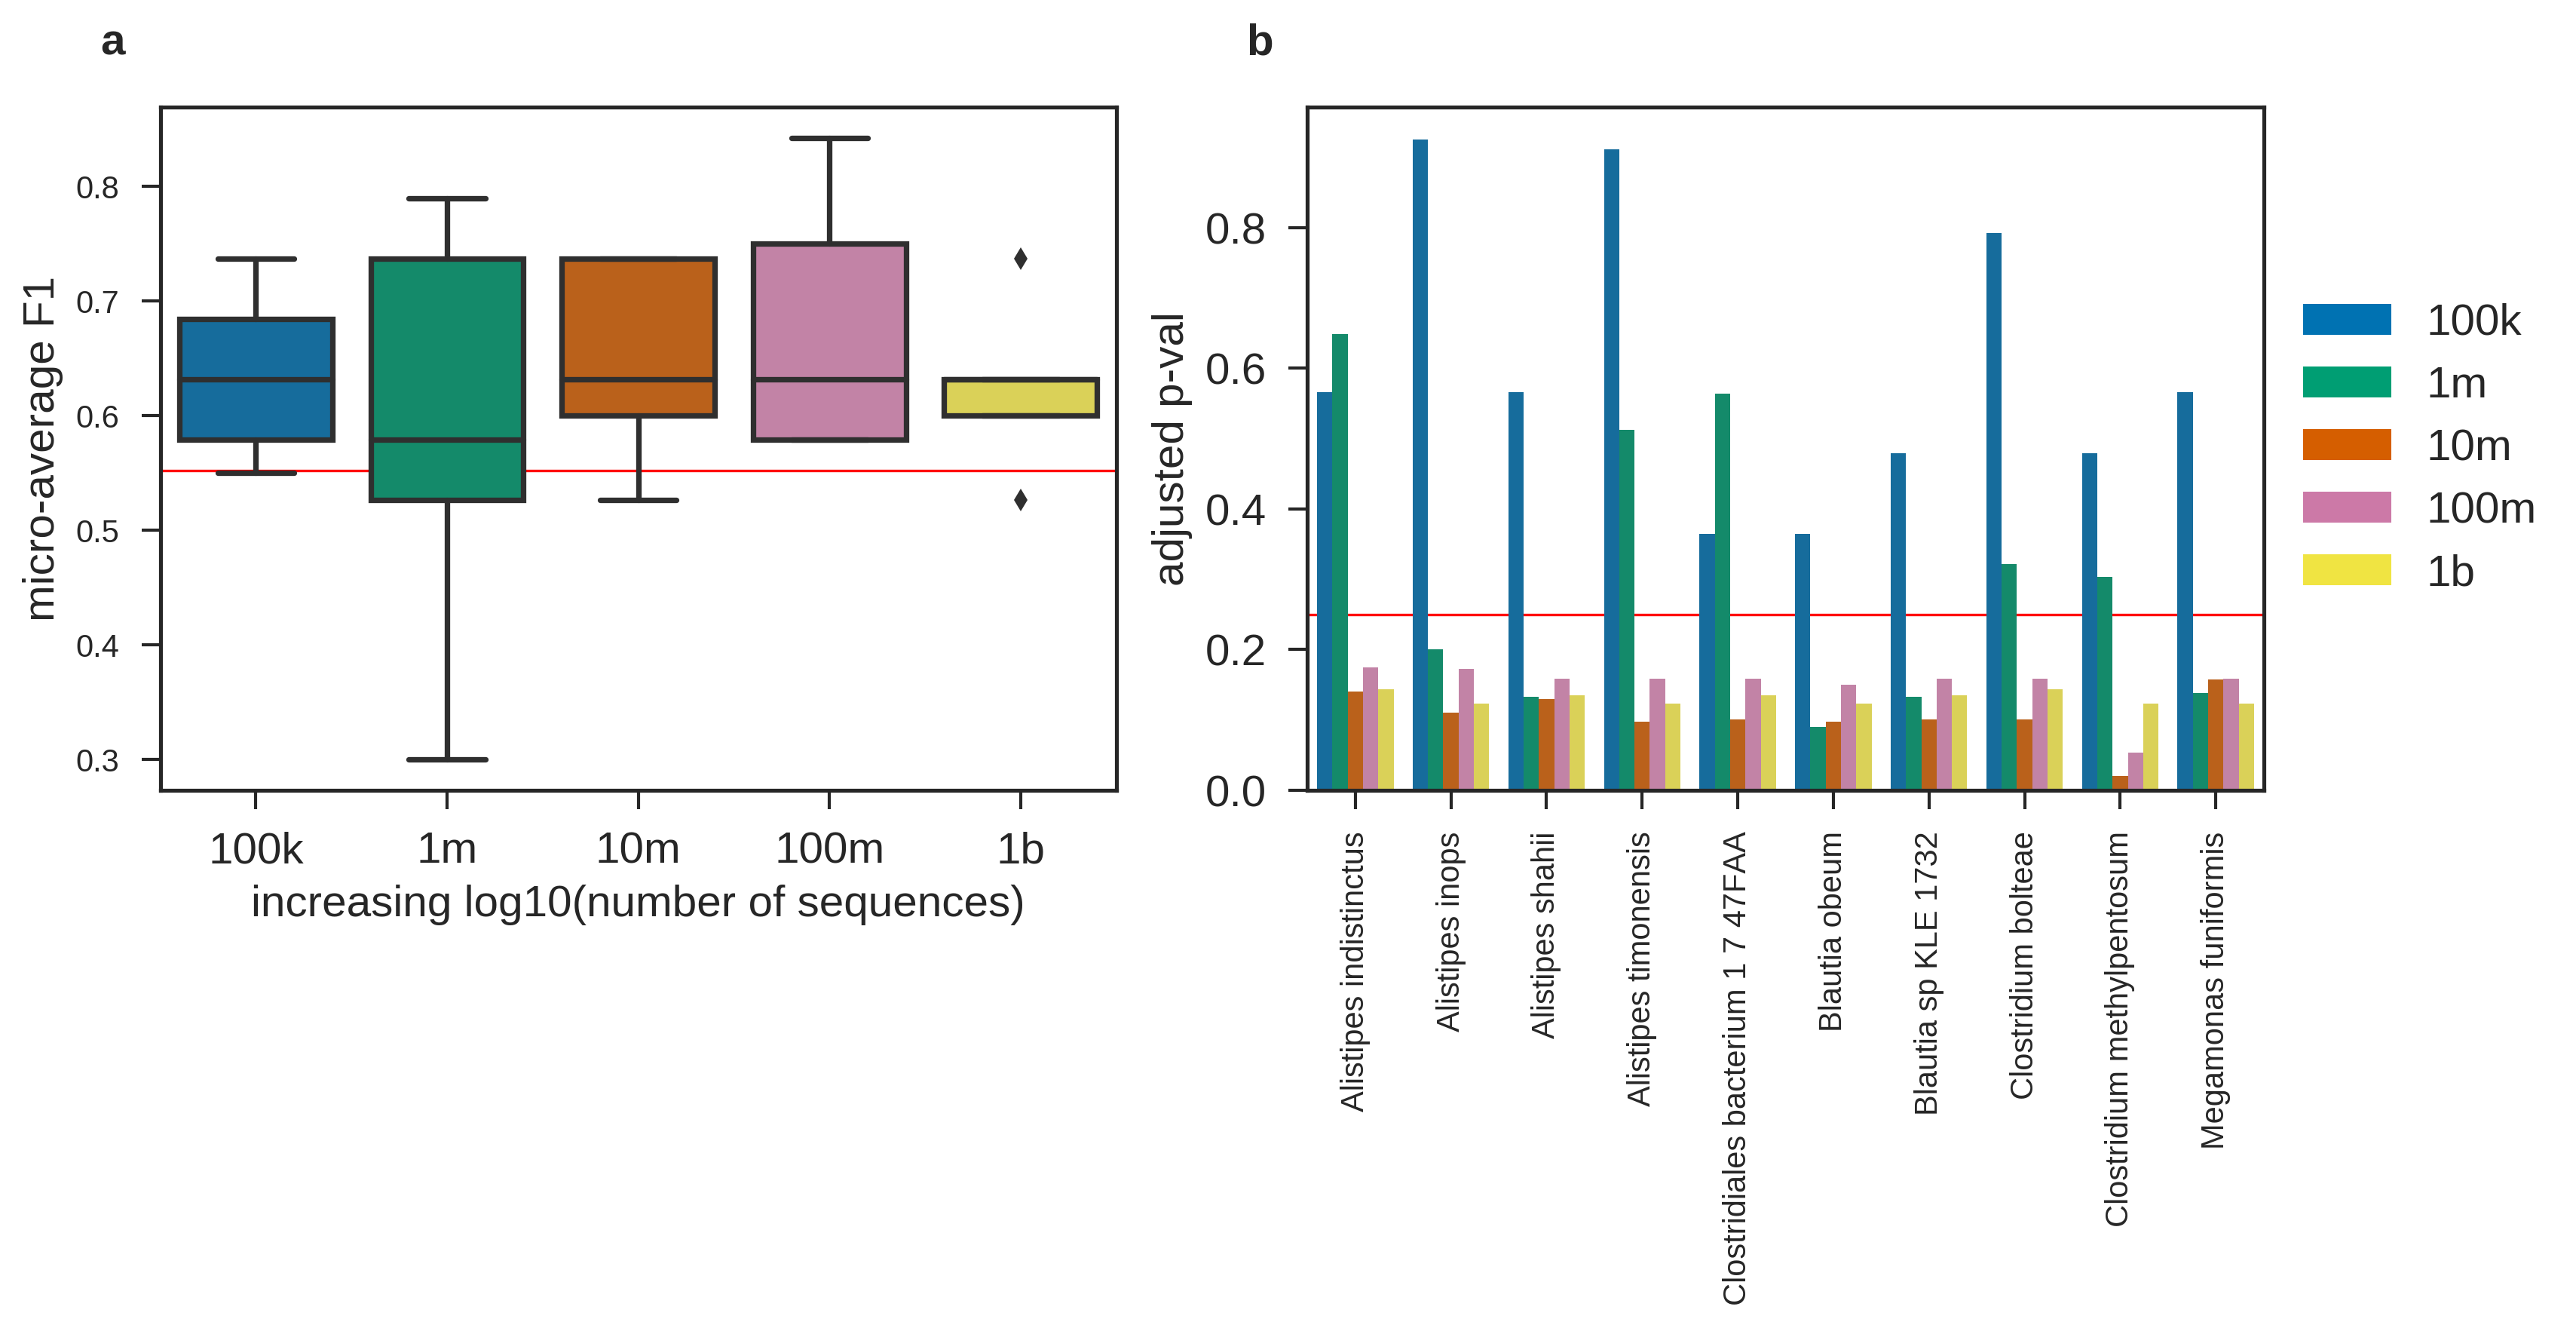
\includegraphics[width=0.8\linewidth]{fig/karlsson2013_f1_combined.png}
    \caption{(a) Raw reads from the sequencing machine are demultiplexed into individual samples. Then, each read is quality controlled with by removing adapters, low quality bases and contaminates such as host reads \cite{consortium_structure_2012}. Optionally, the read pairs can be stitched \cite{magoc_flash:_2011}. (b) The quality-controlled reads are aligned against a database of known genomes to identify each read's most likely source taxon \cite{langmead_fast_2012}. (c) The taxa that are hit are filtered out and summarized at a specific level. These processing steps include last common ancestor assignment \cite{hong_pathoscope_2014}, genome coverage analysis \cite{wood_kraken:_2014}, and redistribution of reads to a specific taxonomic level \cite{lu_bracken:_2017}. (d) After the taxonomic prediction is set, the full functional repertoire of genes is directly observed through a bag-of-genes approach or predicted through a per microbe approach \cite{langille_predictive_2013}.}
      \label{fig:karlsson2013_f1_combined}
\end{figure}

%%% fig:simulations
\begin{figure}[hbt]
    \centering
    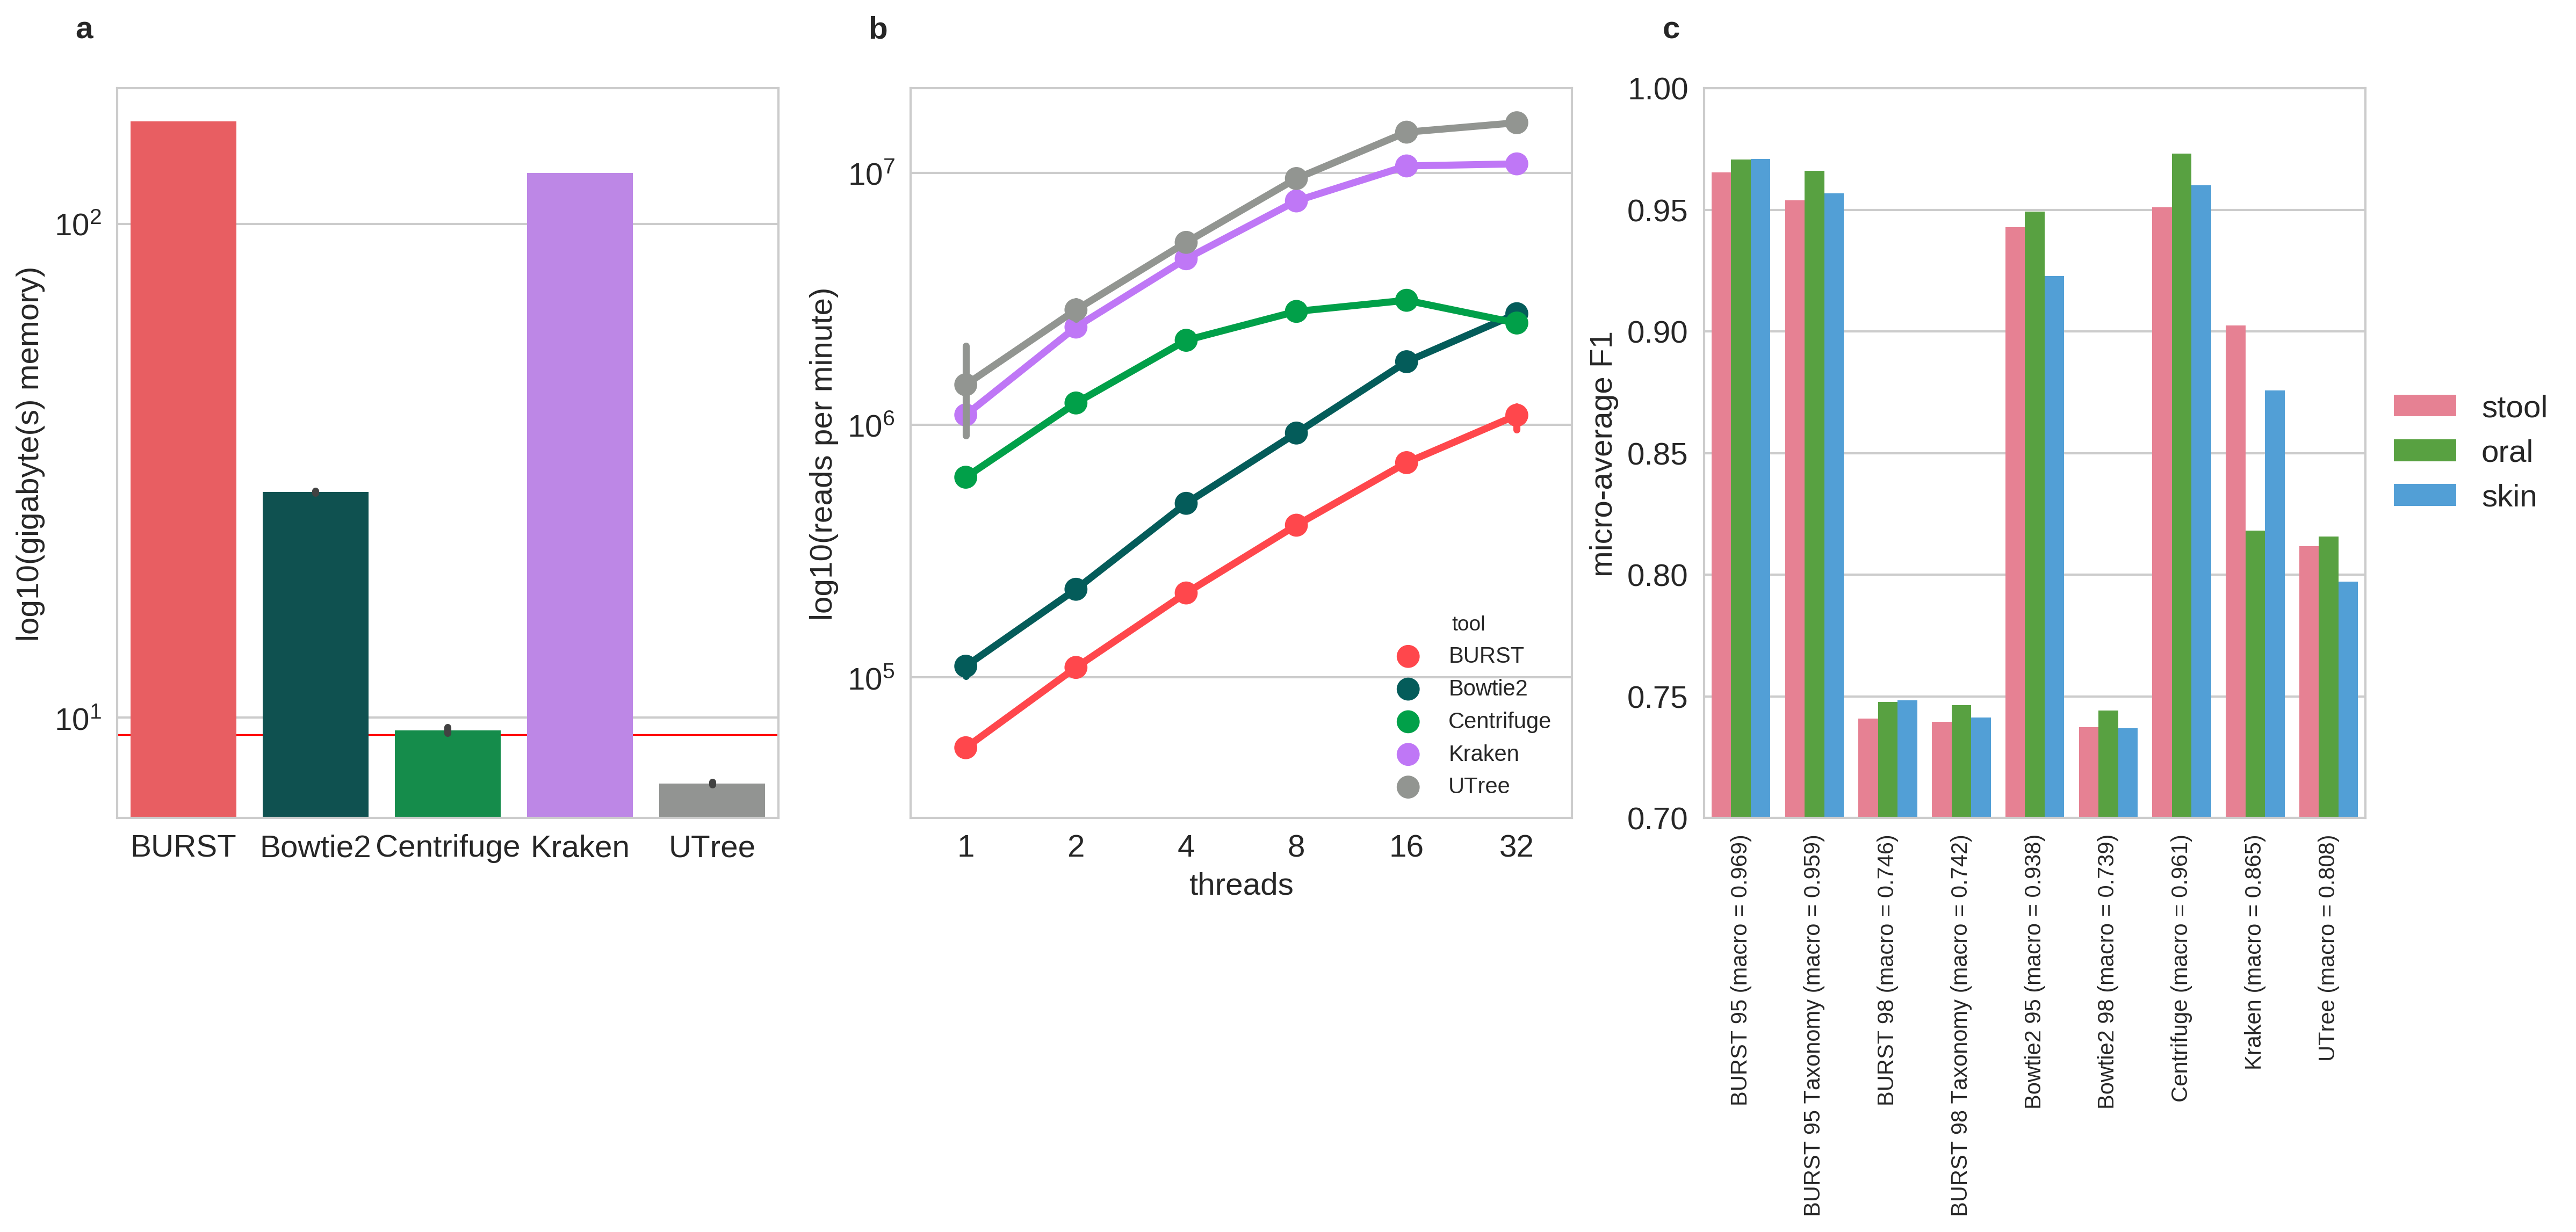
\includegraphics[width=0.8\linewidth]{fig/simulations.png}
    \caption{(a) Raw reads from the sequencing machine are demultiplexed into individual samples. Then, each read is quality controlled with by removing adapters, low quality bases and contaminates such as host reads \cite{consortium_structure_2012}. Optionally, the read pairs can be stitched \cite{magoc_flash:_2011}. (b) The quality-controlled reads are aligned against a database of known genomes to identify each read's most likely source taxon \cite{langmead_fast_2012}. (c) The taxa that are hit are filtered out and summarized at a specific level. These processing steps include last common ancestor assignment \cite{hong_pathoscope_2014}, genome coverage analysis \cite{wood_kraken:_2014}, and redistribution of reads to a specific taxonomic level \cite{lu_bracken:_2017}. (d) After the taxonomic prediction is set, the full functional repertoire of genes is directly observed through a bag-of-genes approach or predicted through a per microbe approach \cite{langille_predictive_2013}.}
      \label{fig:simulations}
\end{figure}

%%% fig:simulations_js
\begin{figure}[hbt]
    \centering
    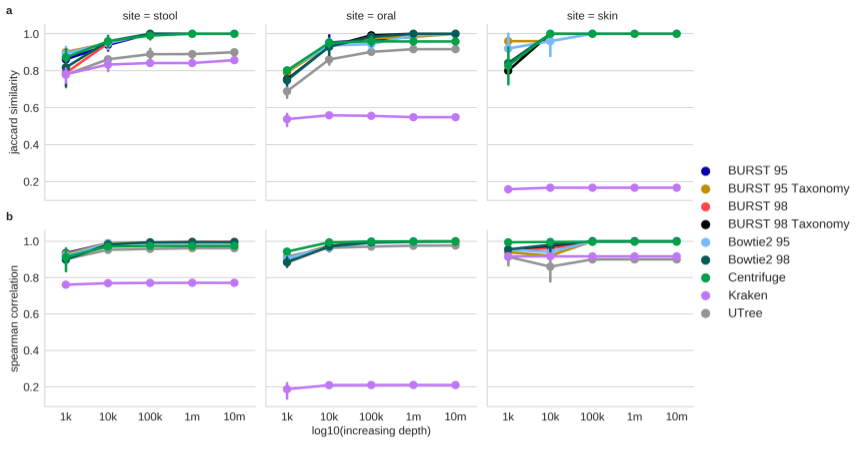
\includegraphics[width=0.8\linewidth]{fig/simulations_js.png}
    \caption{(a) Raw reads from the sequencing machine are demultiplexed into individual samples. Then, each read is quality controlled with by removing adapters, low quality bases and contaminates such as host reads \cite{consortium_structure_2012}. Optionally, the read pairs can be stitched \cite{magoc_flash:_2011}. (b) The quality-controlled reads are aligned against a database of known genomes to identify each read's most likely source taxon \cite{langmead_fast_2012}. (c) The taxa that are hit are filtered out and summarized at a specific level. These processing steps include last common ancestor assignment \cite{hong_pathoscope_2014}, genome coverage analysis \cite{wood_kraken:_2014}, and redistribution of reads to a specific taxonomic level \cite{lu_bracken:_2017}. (d) After the taxonomic prediction is set, the full functional repertoire of genes is directly observed through a bag-of-genes approach or predicted through a per microbe approach \cite{langille_predictive_2013}.}
      \label{fig:simulations_js}
\end{figure}

\subsubsection{Taxonomy} 

\subsubsection{UTree}

\subsubsection{Capitalist}

\subsubsection{Redistribute}

\subsection{Datasets}

\section{Results}

\section{Discussion}

% Table generated by Excel2LaTeX from sheet 'Sheet1'
\begin{table}[htbp]
  \centering
  \caption{Add caption}
    \begin{tabular}{rrll}
    \multicolumn{1}{l}{\textit{Approach}} & \multicolumn{1}{l}{\textit{Examples}} & \textit{Pros} & \textit{Cons} \\
    \midrule
    \midrule
    \multicolumn{1}{l}{\textbf{Last Common Ancestor Alignment}} & \multicolumn{1}{l}{Bowtie2 Taxonomy} & Highest Precision & High RAM \\
          & \multicolumn{1}{l}{BURST Taxonomy} &       & \multicolumn{1}{p{9.5em}}{Slow} \\
          &       &       & No coverage analysis \\
    \midrule
    \multicolumn{1}{l}{\textbf{Exhaustive Alignment}} & \multicolumn{1}{l}{BURST Capitalist} & Highest F1 Accuracy & High RAM \\
          &       & Highest Recall & Slow \\
    \midrule
    \multicolumn{1}{l}{\textbf{Marker Gene}} & \multicolumn{1}{l}{Metaphlan} & Low RAM & No Custom Database \\
          &       & Fast  &  \\
    \midrule
    \multicolumn{1}{l}{\textbf{Exact K-mers}} &       & Fastest & No coverage analysis \\
          &       &       & Sensitive to indels \\
    \cdashlinelr{2-4}
          & \multicolumn{1}{l}{Kraken} &       & High RAM \\
          &       &       & Large Database \\
    \cdashlinelr{2-4}
          & \multicolumn{1}{l}{Utree} & Lowest RAM &  \\
          &       & Smallest Database &  \\
    \midrule
    \multicolumn{1}{l}{\textbf{Longest Common Substring}} & \multicolumn{1}{l}{Centrifuge} & Fast  & No coverage analysis \\
          &       & Low RAM & Sensitive to indels \\
    \end{tabular}%
  \label{tab:addlabel}%
\end{table}%

\subsection{Conclusion}

We recommend that microbiome scientists studying human stool, skin or oral microbiomes use shallow shotgun sequencing instead of amplicon sequencing for large-scale studies.

%\onecolumn
%\section{Appendix A}

\bibliography{Zotero}
\bibliographystyle{IEEEtran}

\end{document}

